\section{Dataset Understanding and Visualization}

\subsection{CREMA Dataset}

For this project, we used the CREMA (Crowd-sourced Emotional Multimodal Actors) dataset, which is widely used in speech emotion recognition research. The dataset consists of audio recordings from 91 actors (48 male, 43 female) with diverse ethnic backgrounds, expressing six basic emotions:

\begin{itemize}
    \item Sadness (SAD)
    \item Anger (ANG)
    \item Disgust (DIS)
    \item Fear (FEA)
    \item Happiness (HAP)
    \item Neutral (NEU)
\end{itemize}

The dataset contains 7,442 audio clips in total, with each clip labeled with the corresponding emotion. The filenames in the CREMA dataset follow a specific format that encodes information about the speaker and emotion: 

\texttt{[ActorID]\_[Sentence]\_[Emotion]\_[Intensity].wav}

For example, \texttt{1001\_AAA\_SAD\_XX.wav} represents a recording from Actor 1001, speaking sentence AAA with sad emotion at regular intensity (XX).

\subsection{Audio Waveform Visualization}

To better understand the dataset, we extracted and visualized sample audio waveforms from each emotion category. Figure \ref{fig:waveforms} shows example waveforms from each of the six emotion classes.
\begin{figure}[h]
    \centering
    \begin{subfigure}[b]{0.32\textwidth}
        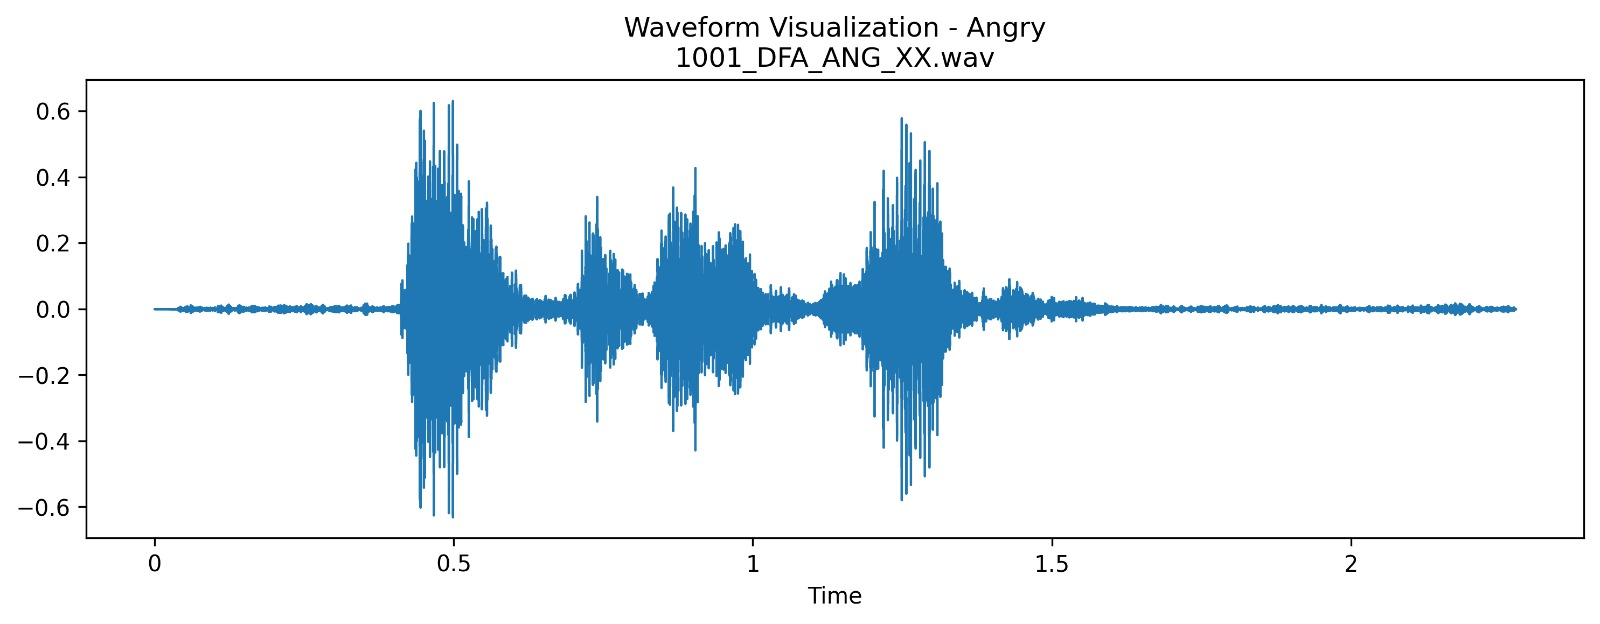
\includegraphics[width=\textwidth]{images/anger.jpeg}
        \caption{Anger}
    \end{subfigure}
    \begin{subfigure}[b]{0.32\textwidth}
        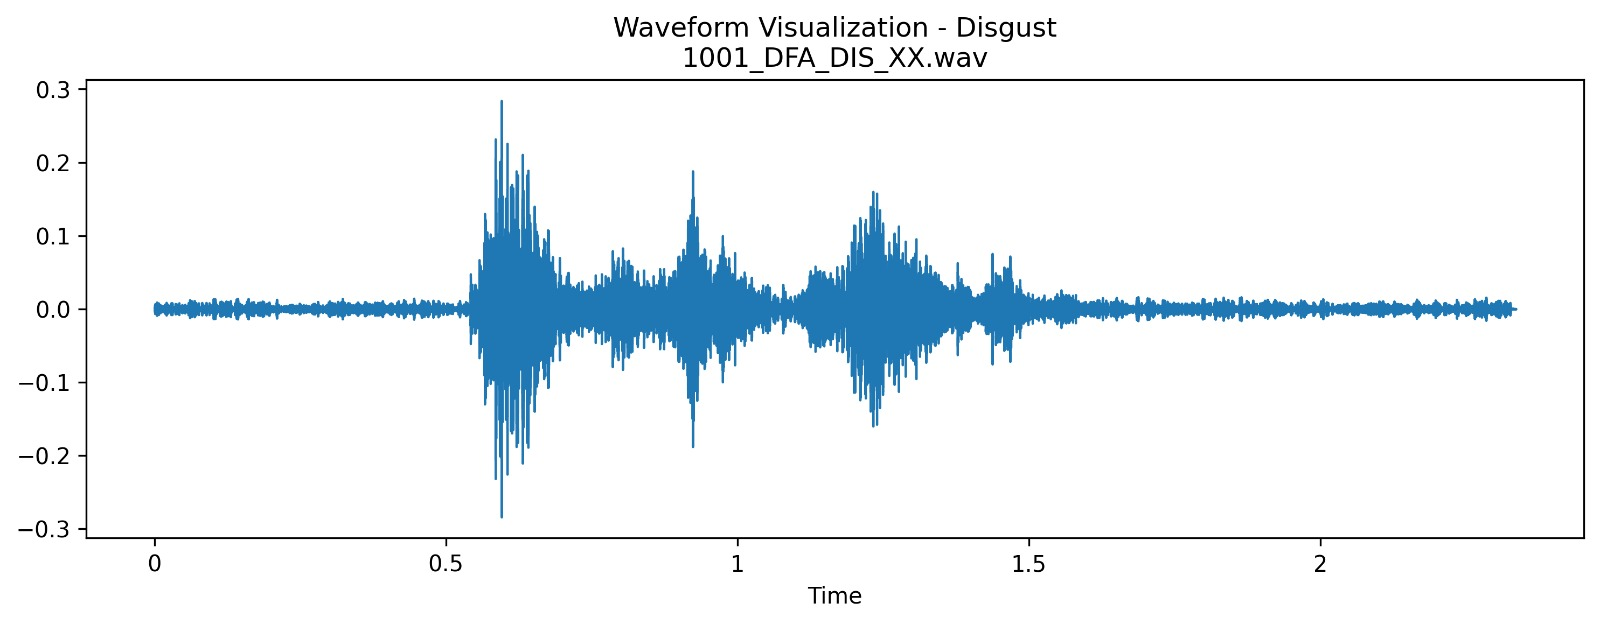
\includegraphics[width=\textwidth]{images/disgust.jpeg}
        \caption{Disgust}
    \end{subfigure}
    \begin{subfigure}[b]{0.32\textwidth}
        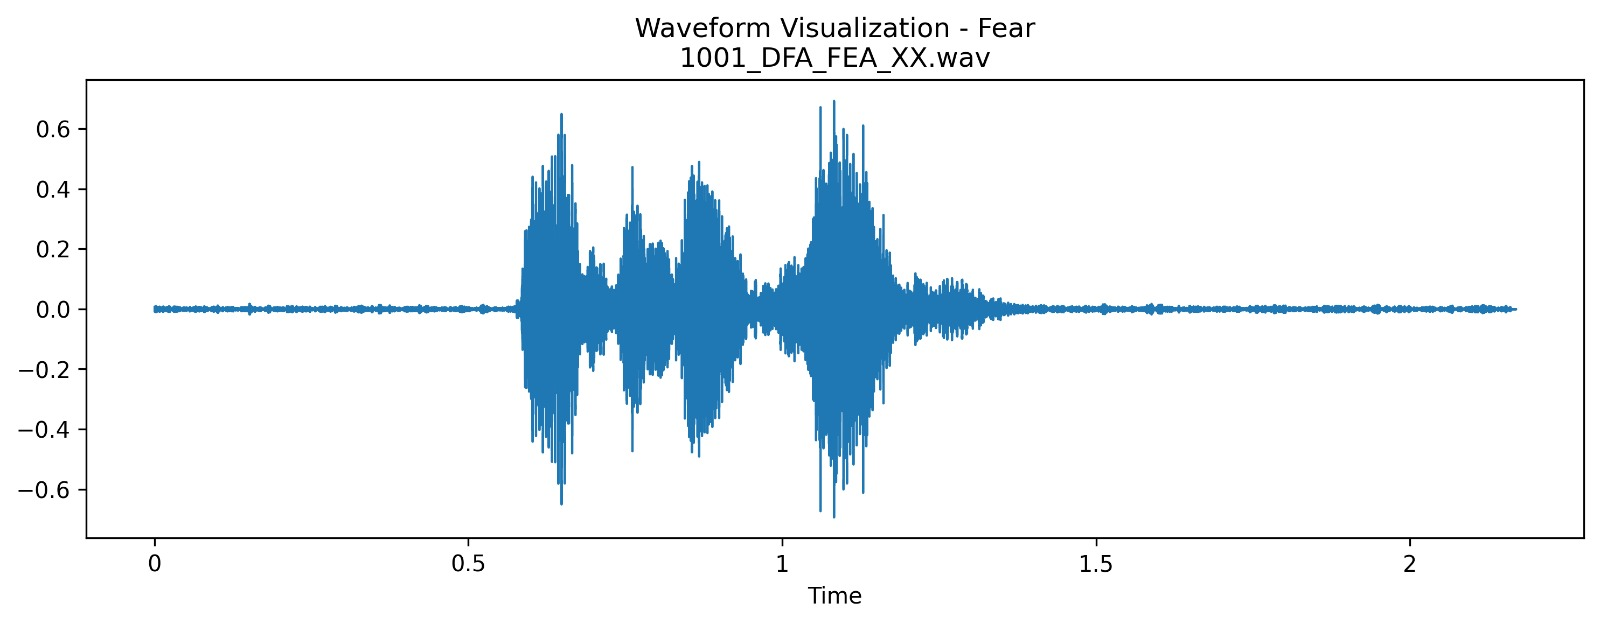
\includegraphics[width=\textwidth]{images/fear.jpeg}
        \caption{Fear}
    \end{subfigure}
    
    \begin{subfigure}[b]{0.32\textwidth}
        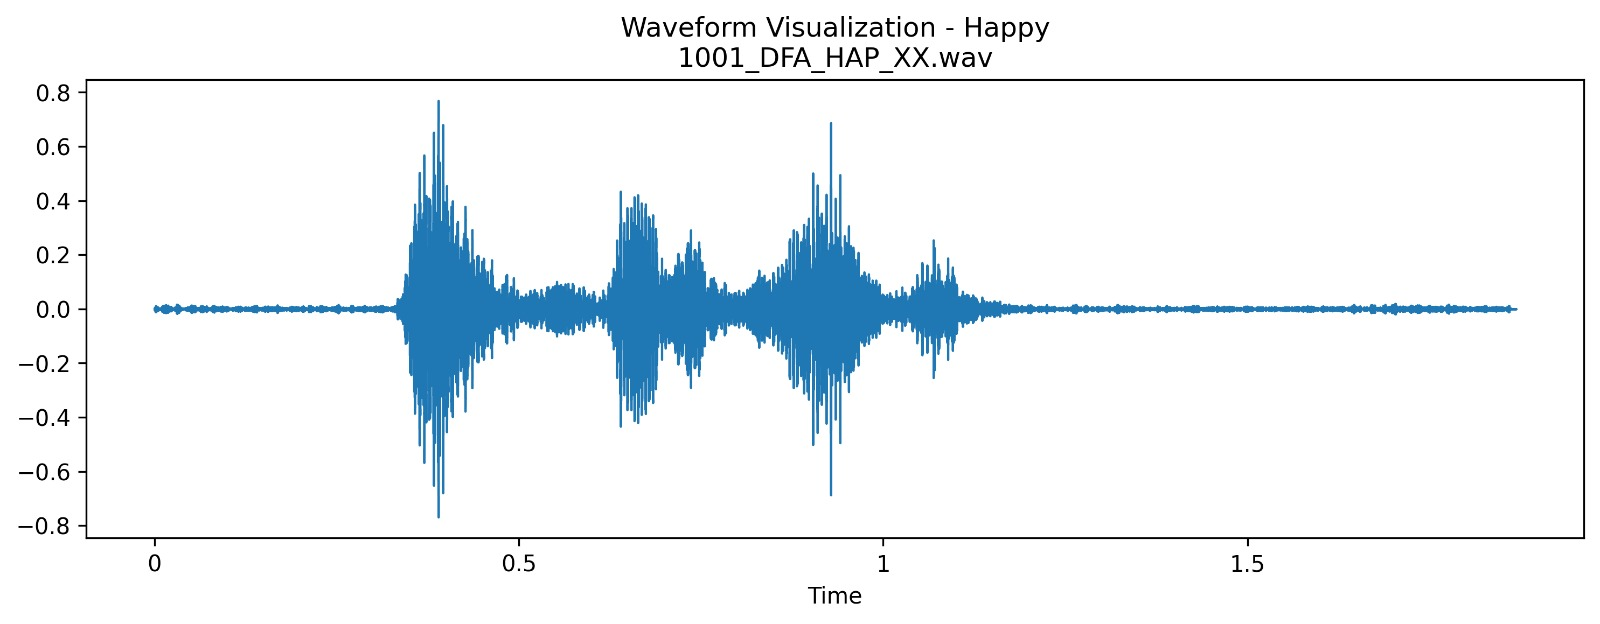
\includegraphics[width=\textwidth]{images/happy.jpeg}
        \caption{Happiness}
    \end{subfigure}
    \begin{subfigure}[b]{0.32\textwidth}
        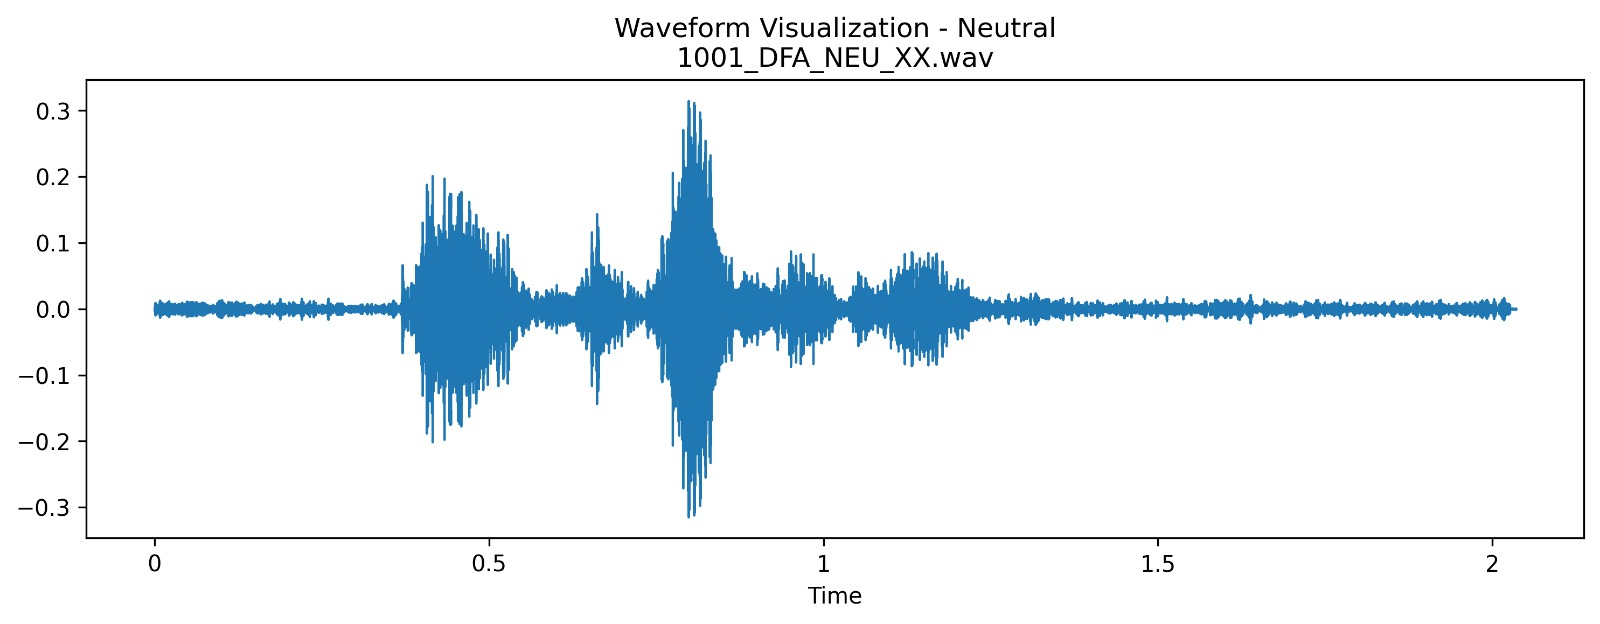
\includegraphics[width=\textwidth]{images/neutral.jpeg}
        \caption{Neutral}
    \end{subfigure}
    \begin{subfigure}[b]{0.32\textwidth}
        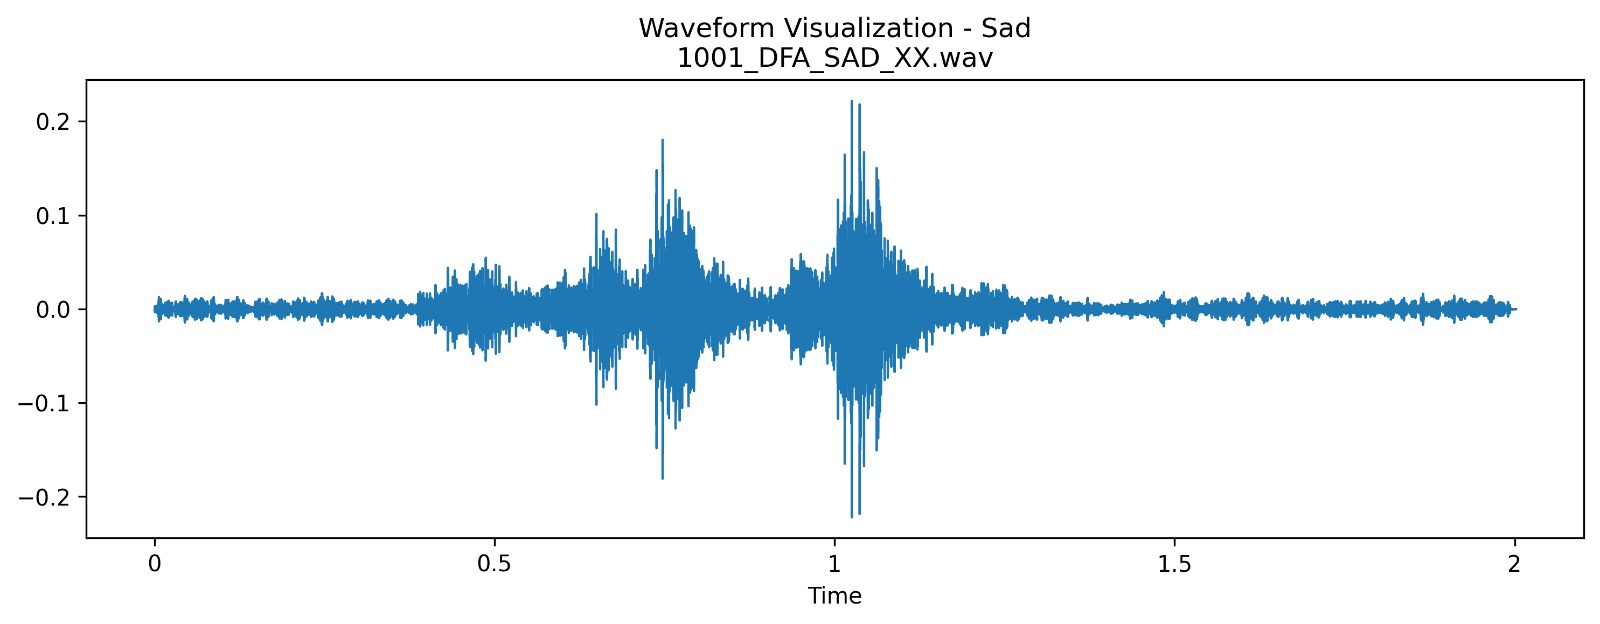
\includegraphics[width=\textwidth]{images/sad.jpeg}
        \caption{Sadness}
    \end{subfigure}
    \caption{Sample waveforms from the CREMA dataset for each emotion class. Notice the variations in amplitude patterns and signal density across different emotional expressions.}
    \label{fig:waveforms}
\end{figure}

\subsection{Audio Preprocessing}

Before feature extraction, we applied several preprocessing steps to prepare the raw audio data:

\begin{itemize}
    \item Conversion to mono channel: All stereo recordings were converted to mono by averaging the channels
    \item Resampling: All audio was resampled to 16kHz for consistency
    \item Voice Activity Detection (VAD): Applied to remove silence and improve signal-to-noise ratio
    \item Normalization: Z-score normalization was applied to standardize signal amplitude
\end{itemize}

These preprocessing steps ensured that our models would be learning from the emotional content rather than variations in recording quality or silence periods. 